\documentclass{report}
\usepackage[T1]{fontenc} % Fontes T1
\usepackage[utf8]{inputenc} % Input UTF8
\usepackage[backend=biber, style=ieee]{biblatex} % para usar bibliografia
\usepackage{csquotes}
\usepackage[portuguese]{babel} %Usar língua portuguesa
\usepackage{blindtext} % Gerar texto automaticamente
\usepackage[printonlyused]{acronym}
\usepackage{hyperref} % para autoref
\usepackage{graphicx}
\usepackage{indentfirst}
\bibliography{bibliografia}


\begin{document}
%%
% Definições
%
\def\titulo{Sistemas de Armazenamento de Dados}
\def\data{14/11/2017}
\def\autores{Afonso Cardoso, Pedro Almeida}
\def\autorescontactos{(88964) afonsocardoso@ua.pt, (89205) pedro22@ua.pt}
\def\versao{VERSAO}
\def\departamento{Departamento de Electrónica, Telecomunicações e Informática}
\def\empresa{Universidade De Aveiro}
\def\logotipo{ua.pdf}
%
%%%%%% CAPA %%%%%%
%
\begin{titlepage}

\begin{center}
%
\vspace*{50mm}
%
{\Huge \titulo}\\ 
%
\vspace{10mm}
%
{\Large \empresa}\\
%
\vspace{10mm}
%
{\LARGE \autores}\\ 
%
\vspace{30mm}
%
\begin{figure}[h]
\center
\includegraphics{\logotipo}
\end{figure}
%
\vspace{30mm}
\end{center}
%
\begin{flushright}
\versao
\end{flushright}
\end{titlepage}

%%  Página de Título %%
\title{%
{\Huge\textbf{\titulo}}\\
{\Large \departamento\\ \empresa}
}
%
\author{%
    \autores \\
    \autorescontactos
}
%
\date{\data}
%
\maketitle

\pagenumbering{roman}

%%%%%% RESUMO %%%%%%
\begin{abstract}
Resumo de 200-300 palavras.
\end{abstract}

%%%%%% Agradecimentos %%%%%%
% Segundo glisc deveria aparecer após conclusão...
\renewcommand{\abstractname}{Agradecimentos}
\begin{abstract}
Eventuais agradecimentos.
Comentar bloco caso não existam agradecimentos a fazer.
\end{abstract}

\tableofcontents
% \listoftables     % descomentar se necessário
% \listoffigures    % descomentar se necessário


%%%%%%%%%%%%%%%%%%%%%%%%%%%%%%%
\clearpage
\pagenumbering{arabic}

%%%%%%%%%%%%%%%%%%%%%%%%%%%%%%%%
\chapter{Introdução}
\label{chap.introducao}
%Introduz o tema, apresenta a motivação e finalmente a estrutura.
	Com a evolução da tecnologia e o surgimento das primeiras invenções mecanizadas, surgiu a necessidade de guardar dados e informações importantes. Assim, como resposta a este problema, teve de ser criado algo com a capacidade de registar e guardar essa informação. O que foi criado foram dispositivos de armazenamento de dados, sendo o primeiro o \textit{Punched card} (Cartão perfurado), utilizado pela primeira vez em 1725. 
\vspace{1mm}
	
	Contudo, na atualidade, o armazenamento de dados não é utilizado apenas pelas industrias mas também para utilização pessoal. Todos sentem a necessidade de guardar algo, seja qual for a utilidade ou fim. "Dados são conhecimento, é um pedaço de história, um fragmento de algo ou um todo de uma vida"[1].
\vspace{1mm}
	
	Estes dispositivos de armazenamento têm vindo a sofrer um processo de evolução ininterrupto até aos dias de hoje. Tendo sempre como base as suas origens e como visão, o aumento da sua capacidade de armazenamento, o aumento da velocidade de acesso à informação guardada, assim como, a redução das dimensões físicas dos sistemas de armazenamento.
\vspace{1mm}
	
	Uma alteração que acontece na atualidade em novos computadores, é a substituição do muito usado e comum disco rígido pelo \textit{solid-state drive} (SSD). Assim como este exemplo dado, houve muitas outras inovações que levaram a tecnologia anterior a entrar em desuso, como irá ser descrito com mais pormenor mais à frente.
\vspace{1mm}
%motivaçao	

	Estas evoluções e mudanças na área do armazenamento de dados foi, sem dúvida, o que despertou o interesse para a elaboração deste trabalho, pretendendo, assim, descobrir a origem e a história destes sistemas até aos dias de hoje.
\vspace{2mm}



Este documento está dividido em quatro capítulos.
Depois desta introdução,
no \autoref{chap.metodologia} é apresentada a metodologia seguida,
no \autoref{chap.resultados} são apresentados os resultados obtidos,
sendo estes discutidos no \autoref{chap.analise}.
Finalmente, no \autoref{chap.conclusao} são apresentadas
as conclusões do trabalho.

\chapter{Metodologia}
\label{chap.metodologia}
Descreve os métodos utilizados para obtenção de resultados.

Neste esqueleto de relatório aproveitamos este capítulo para exemplificar
como se usam alguns elementos de {\LaTeX}.

\section{Exemplos}

\subsection{Utilização de acrónimos}
Esta é a primeira invocação do acrónimo \ac{ua}.
E esta é a segunda: \ac{ua}.

Outras duas referências a \ac{miect}
e \ac{miect}.

\subsection{Referências bibliográficas}
Informação relativa à estrutura formal de um relatório pode ser obtida
na página do \ac{glisc}\cite{glisc}.

\chapter{Conteúdo}
\label{chap.conteúdo}
	\section{História de Sistemas de Armazenamento de Dados}
		\subsection{Cartão Perfurado}
		O Cartão Perfurado(\textit{Punched Card} foi inventado por Joseph-Marie Jacquard em 1804 para o comando automático de teares depois de ter percebido que as mudanças de linhas coloridas e novelos  seguiam uma certa lógica. Deste modo, Jacquard inventou um processo de cartões perfurados que definiam padrões nas lançadeiras e assim o trabalho do tecelão seria trocado para algo "automático". 
		
		Os cartões perfurados contêm informações digitais representadas pela presença ou falta de furos em posições predefinidas. O método foi interessante para codificar as informações e do ano 1900 a 1950, foram o principal meio de entrada de dados, armazenamento de dados e processamento na computação institucional, tudo pela mão da \textit{International Business Machines} (IBM). 
		
		Apesar de várias melhorias ao longo dos anos, com o desenvolver das tecnologias, os cartões perfurados não conseguiam suprir as necessidades e acabaram por ser substituídos.
		
		\begin{figure}[h]
		\centering
		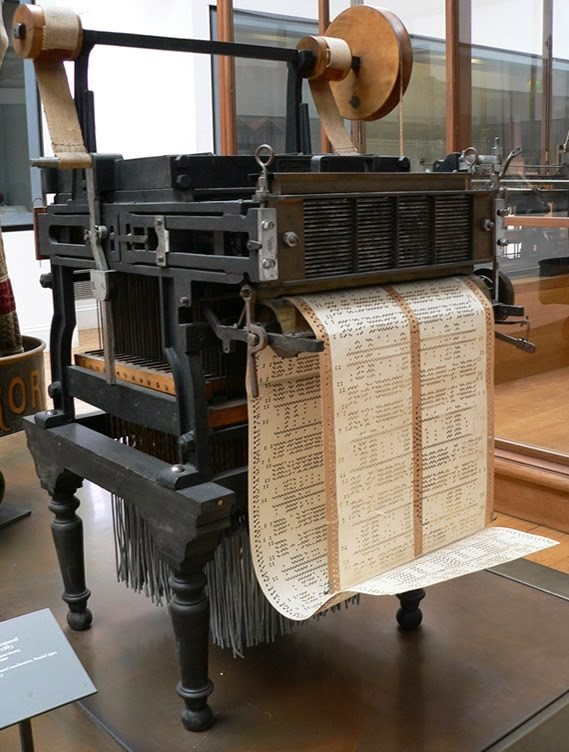
\includegraphics[width=3cm, height=4cm]{cartaoperfurado.jpg}
		\caption{Cartão Perfurado}
		\end{figure}
\newpage

		\subsection{Tubo de Williams}
		O Tubo de Williams é um tipo de memória para computadores criada por Sir Frederick Williams no ano de 1947 na Universidade Manchester tendo sido usado dois anos mais tarde na construção do computador Manchester Mark I.
	
	Este foi o primeiro dispositivo digital de memória de acesso aleatório e foi utilizado com sucesso em vários computadores antigos e possuía uma velocidade de 1,2 milésimos de segundo por instrução, o que na altura era algo bastante inovador.
	
	No seu processo de armazenamento de informação, um eletrão percorre sucessivas linhas na face do tubo, marcando com pontos ou traços de carga elétrica florescente na placa representando assim os uns e os zeros do código binário.
	
	Os primeiros computadores utilizavam este tipo de memória de tubos de raios catódicos (feixes de eletrões), díodo-condensador (mantém a corrente a circular apenas num sentido) e também as memórias de linha de retardo que consistiam num tubo de aproximadamente 150 cm de comprimento contendo mercúrio, com um cristal de quartzo em cada ponta onde os dados a armazenar passavam pelo mercúrio na forma de vibrações mecânicas e eram reconvertidos na outra ponta.
	
	
		\subsection{Tambor de Memória}
		 O tambor de memória, também conhecido como\textit{ Drum Memory} foi inventado por Gustav Tauschek em 1932 na Áustria e foi amplamente usado na década de 1950 e na década de 1960.
		 O tambor magnético é constituído por um cilindro de revolução metálico que roda em torno de um eixo vertical e o movimento é assegurado por um motor elétrico. Um conjunto de cabeças fixas assegura a gravação e a leitura da informação
		 
		 A capacidade de armazenamento do tambor de memória original tinha uma capacidade de cerca de 500,000 bits. Este sistema de armazenamento de dados foi especialmente importante pois, no início da década de 60 passaram a utilizar-se na construção de computadores com memórias não voláteis, isto é, não perde a informação guardada depois de desligar a fonte de energia. Estas memórias eram construídas com ferrites e marcam um grande avanço tecnológico na área do armazenamento de dados.
	
	\begin{figure}[h]
		\centering
		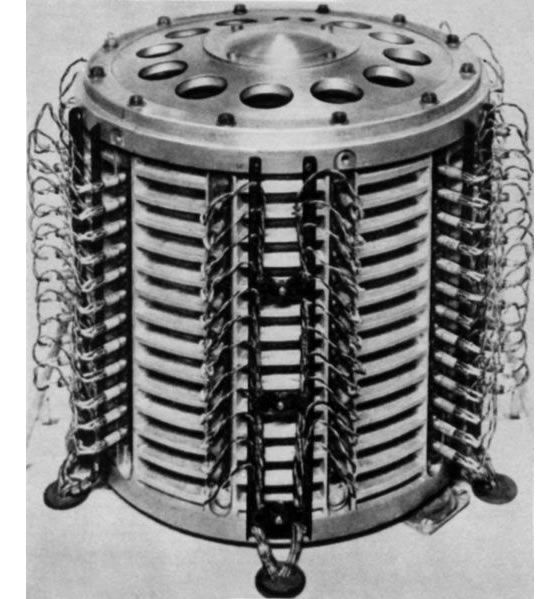
\includegraphics[width=3cm, height=4cm]{tambordememoria.jpg}
		\caption{Tambor de Memória}
		\end{figure}
\newpage

		\subsection{IBM 350 Disk Storage Unit}
		Em 1956, a IBM lançou no mercado o IBM 305 RAMAC(\textit{(Random Access Method of Accounting and Control}), o primeiro computador produzido em série para empresas, visto que até aqui, os computadores eram exclusivos para aplicações militares. Assim, o RAMAC, foi projetado para executar aplicativos de contabilidade e controlo de transações comercias, tais como processamento de pedidos, controlo de inventário e folhas de pagamentos.
		
		A novidade que o computador 305 RAMAC, que era equipado com 350 Disk Storage Unit, não era a sua capacidade de processamento, mas na utilização de um novo equipamento periférico para a entrada e saída de dados, o qual permitia a gravação e leitura de dados de forma muito mais rápida comparada com os outros sistemas de armazenamento usados até então.
		
		
	
%\chapter{Análise}
%\label{chap.analise}
%Analisa os resultados.

\chapter{Conclusões}
\label{chap.conclusao}
Apresenta conclusões.

\chapter*{Contribuições dos autores}
Resumir aqui o que cada autor fez no trabalho.
Usar abreviaturas para identificar os autores,
por exemplo AS para António Silva.
No fim indicar a percentagem de contribuição de cada autor.

%%%%%%%%%%%%%%%%%%%%%%%%%%%%%%%%%
\chapter*{Acrónimos}
\begin{acronym}
\acro{ua}[UA]{Universidade de Aveiro}
\acro{miect}[MIECT]{Mestrado Integrado em Engenharia de Computadores e Telemática}
\acro{lei}[LEI]{Licenciatura em Engenharia Informática}
\acro{glisc}[GLISC]{Grey Literature International Steering Committee}
\end{acronym}


%%%%%%%%%%%%%%%%%%%%%%%%%%%%%%%%%
\printbibliography

\end{document}
